\documentclass{article}
\usepackage{xcolor}
\usepackage{noto}
\usepackage{hyperref}
\usepackage{graphicx}
\graphicspath{ {./images/} }
\pagenumbering{gobble}

\title{Lettera A}
\author{F.Zanasi}
\date{Ottobre 2023}

\begin{document}

% \maketitle
{\fontsize{200}{210}\selectfont A} 
\\[1cm]
{\fontsize{100}{100}\color{blue}\texttt{A}\color{black}\texttt{PE}} 

\includegraphics[scale=0.5]{flag-IT1}

\includegraphics[scale=0.5]{ape}
\\[3cm]
{\fontsize{100}{110}\color{blue}\texttt{A}\color{black}\texttt{PE}} 

\includegraphics[scale=0.5]{flag-UK}
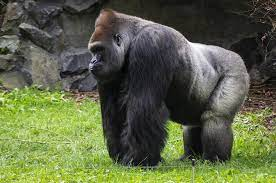
\includegraphics[scale=0.5]{gorilla}



% \section{Introduction}
% This example project uses the \href{https://ctan.org/pkg/noto?lang=en}{\color{blue}\texttt{noto}} package to typeset your document using Google's Noto fonts\footnote{\url{https://www.google.com/get/noto/}}:
% \begin{itemize}
% \item \verb|\textbf{bold}| produces \textbf{bold}
% \item \verb|\textit{italic}| produces \textit{italic}
% \item \verb|\textbf{\textit{bold italic}}| produces \textbf{\textit{bold italic}}
% \item \verb|\emph{emphasis}| produces \emph{emphasis}
% \item \verb|\textbf{\emph{bold italic}}| produces \textbf{\emph{bold italic}}
% \end{itemize}

% \subsection{Monospaced fonts}

% You can use Noto's monospaced fonts for \texttt{regular} and \texttt{\textbf{bold}} monospaced text.

% \subsection{Sans serif fonts}
% Here is some \textsf{text is typeset in a sans serif font} together with \textbf{\textsf{text typeset in bold sans serif}}.

% \section{Further reading}
% Documentation for the \texttt{noto} package can be found in its \href{http://mirrors.ctan.org/fonts/noto/README}{\color{blue}\texttt{readme} file on CTAN}.

\end{document}